
\documentclass{exam}

\usepackage{units} 
\usepackage{graphicx}
\usepackage[fleqn]{amsmath}
\usepackage{cancel}
\usepackage{float}
\usepackage{mdwlist}
\usepackage{booktabs}
\usepackage{cancel}
\usepackage{polynom}
\usepackage{caption}
\usepackage{fullpage}
\usepackage{xfrac}
\usepackage{enumerate}

\newcommand{\degree}{\ensuremath{^\circ}} 
\everymath{\displaystyle}

% \begin{figure}[H]
%   \centering
%   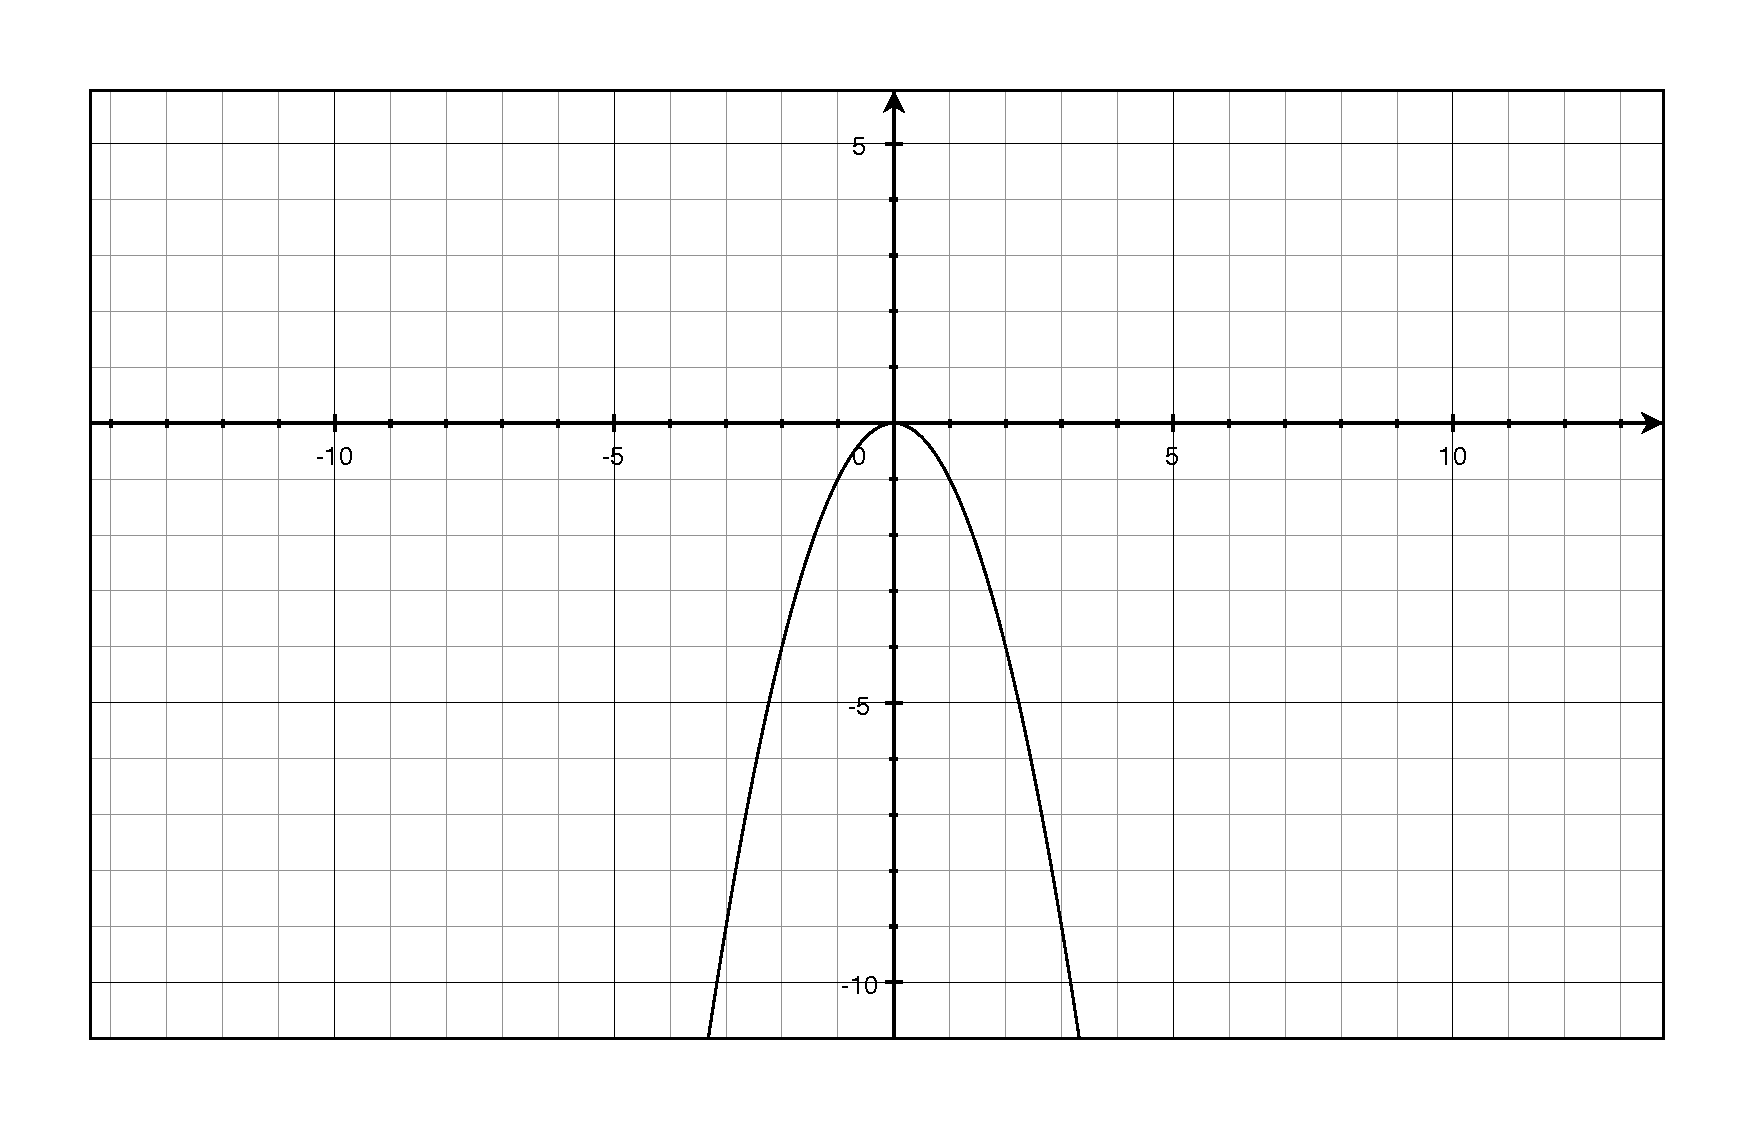
\includegraphics[scale=1.0]{problem7.eps}
%   \caption*{Problem 7}
% \end{figure}

% \begin{tabular}{cc}
%   \toprule
%   period & amplitude \\
%   \midrule
%   value one & value two
%   \bottomrule
% \end{tabular}

\printanswers

\ifprintanswers 
  \usepackage{2in1, lscape} 
\fi

\date{May 15, 2013}
\author{}
\title{Math 141 \\ Homework 13}

\begin{document}

\maketitle


\section{Homework}

\begin{itemize*}
  \item Read Section 4.1 
  \item Section 4.1: 
\end{itemize*}

\section{Extra Credit}
  TO DO 

\ifprintanswers
  \pagebreak

  \begin{description}
    \item[1] TO DO

  \end{description}

  \pagebreak

  \section{Section 4.1}

  \begin{description}

    \item[11] 
      \begin{figure}[H]
        \centering
        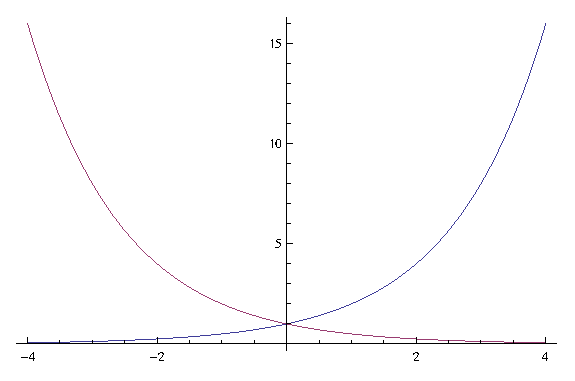
\includegraphics[scale=1.0]{exercise11.eps}
        \caption*{Exercise 11}
      \end{figure}

    \item[12] 
      \begin{figure}[H]
        \centering
        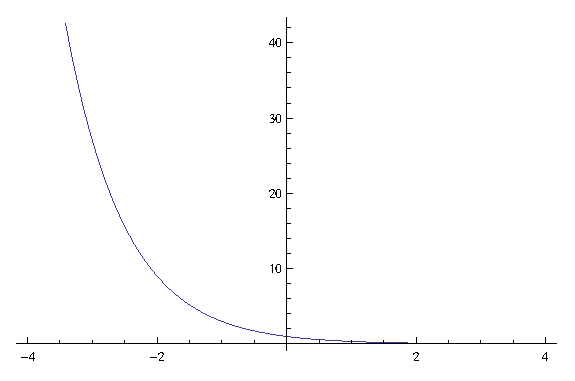
\includegraphics[scale=1.0]{exercise12.eps}
        \caption*{Exercise 12}
      \end{figure}

    \item[15] $f(x) = 3^x$

    \item[16] $f(x) = 5^x$

    \item[17] $f(x) = 4^{-x}$

    \item[18] $f(x) = 2^{-x}$

    \item[19] III

    \item[20] V

    \item[21] I

    \item[22] VI

    \item[23] II

    \item[24] IV

    \item[25] 
      \begin{figure}[H]
        \centering
        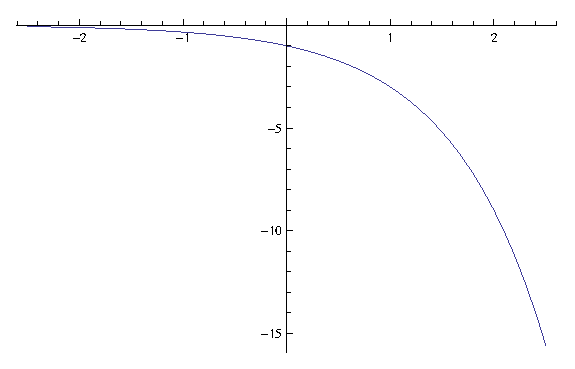
\includegraphics[scale=1.0]{exercise25.eps}
        \caption*{Exercise 25: $f(x) = -3^x$}
      \end{figure}

      \begin{tabular}[H]{ll}
        \toprule
        domain    & $(-\infty, \infty)$ \\
        range     & $(-\infty, 0)$ \\
        asymptote & $x = 0$ \\
        \bottomrule
      \end{tabular}

    \pagebreak

    \item[26] 
      \begin{figure}[H]
        \centering
        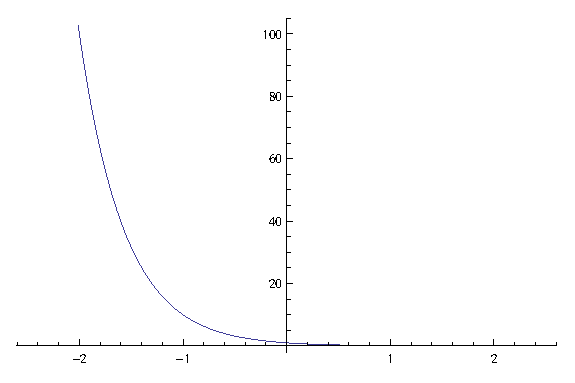
\includegraphics[scale=1.0]{exercise26.eps}
        \caption*{Exercise 26: $f(x) = 10^{-x}$}
      \end{figure}

      \begin{tabular}[H]{ll}
        \toprule
        domain    & $(-\infty, \infty)$ \\
        range     & $(0, \infty)$ \\
        asymptote & $x = 0$ \\
        \bottomrule
      \end{tabular}

    \item[27] 
      \begin{figure}[H]
        \centering
        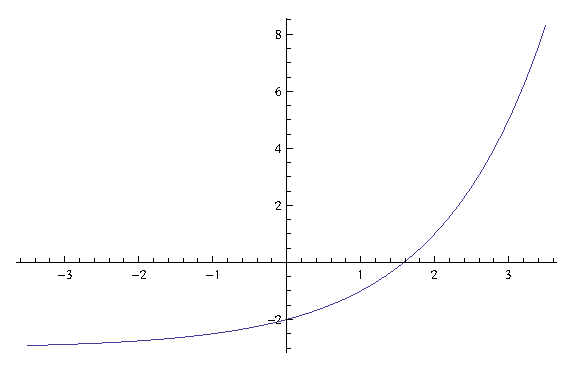
\includegraphics[scale=1.0]{exercise27.eps}
        \caption*{Exercise 27: $g(x) = 2^x - 3$}
      \end{figure}

      \begin{tabular}[H]{ll}
        \toprule
        domain    & $(-\infty, \infty)$ \\
        range     & $(-3, \infty)$ \\
        asymptote & $x = -3$ \\
        \bottomrule
      \end{tabular}

    \item[28] 
      \begin{figure}[H]
        \centering
        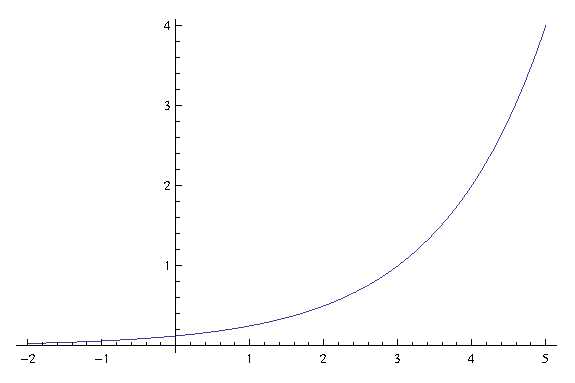
\includegraphics[scale=1.0]{exercise28.eps}
        \caption*{Exercise 28: $g(x) = 2^{x - 3}$}
      \end{figure}

      \begin{tabular}[H]{ll}
        \toprule
        domain    & $(-\infty, \infty)$ \\
        range     & $(-3, \infty)$ \\
        asymptote & $x = 0$ \\
        \bottomrule
      \end{tabular}

    \item[29] 
      \begin{figure}[H]
        \centering
        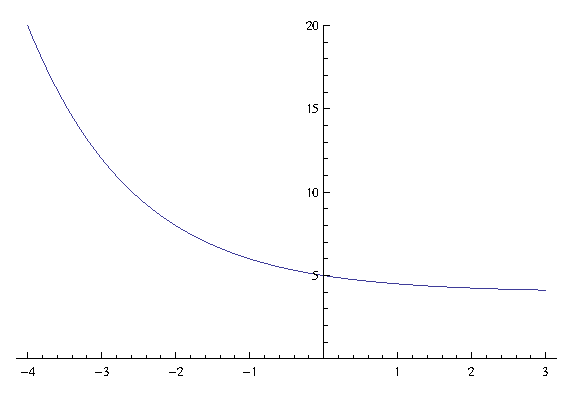
\includegraphics[scale=1.0]{exercise29.eps}
        \caption*{Exercise 29: $g(x) = 4 + \left( \frac{1}{2} \right)^x$}
      \end{figure}

      \begin{tabular}[H]{ll}
        \toprule
        domain    & $(-\infty, \infty)$ \\
        range     & $(-3, \infty)$ \\
        asymptote & $x = 4$ \\
        \bottomrule
      \end{tabular}

    \item[30] 
      \begin{figure}[H]
        \centering
        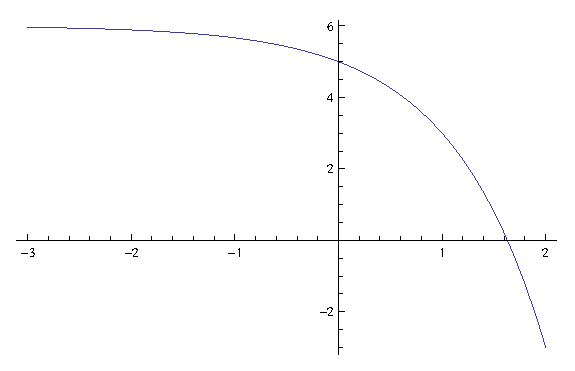
\includegraphics[scale=1.0]{exercise30.eps}
        \caption*{Exercise 30: $g(x) = 6 - 3^x$}
      \end{figure}

      \begin{tabular}[H]{ll}
        \toprule
        domain    & $(-\infty, \infty)$ \\
        range     & $(-\infty, 6)$ \\
        asymptote & $x = 6$ \\
        \bottomrule
      \end{tabular}

    \item[33] 
      \begin{figure}[H]
        \centering
        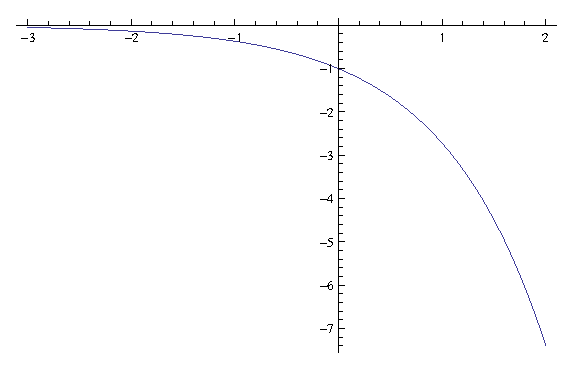
\includegraphics[scale=1.0]{exercise33.eps}
        \caption*{Exercise 33: $g(x) = -e^x$}
      \end{figure}

      \begin{tabular}[H]{ll}
        \toprule
        domain    & $(-\infty, \infty)$ \\
        range     & $(-\infty, 0)$ \\
        asymptote & $x = 0$ \\
        \bottomrule
      \end{tabular}

    \item[34] 
      \begin{figure}[H]
        \centering
        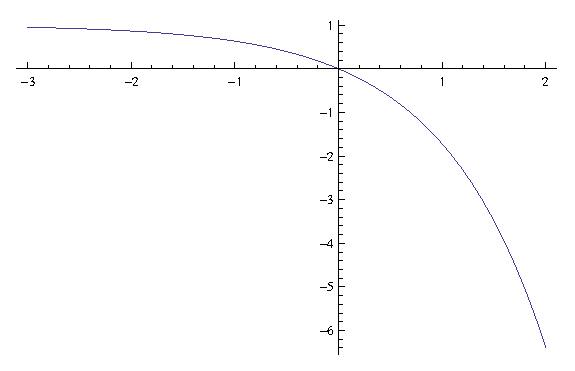
\includegraphics[scale=1.0]{exercise34.eps}
        \caption*{Exercise 34: $g(x) = 1 - e^x$}
      \end{figure}

      \begin{tabular}[H]{ll}
        \toprule
        domain    & $(-\infty, \infty)$ \\
        range     & $(-\infty, 0)$ \\
        asymptote & $x = 0$ \\
        \bottomrule
      \end{tabular}

  \end{description}

\else
  \vspace{6 cm}
  \begin{quote}
    \begin{em}
      to do
    \end{em}
  \end{quote}

  \hspace{1 cm} --author here


\fi

\end{document}

